\chapter{Planification et Roadmap}

% Chapeau du chapitre (Obligatoire selon le modèle du mémoire)
Dans ce chapitre, nous présentons l'organisation du projet au cours du second semestre. Notre travail va se diviser en quatre phases principales, allant de la mise en place technique jusqu'à la rédaction finale. Cette planification assure une progression logique, de la validation des outils à l'interprétation des données neurolinguistiques.

\section{Mise en place de l'environnement technique et Génération des Stimuli (Février)}

L'objectif de cette première phase est de disposer d'un pipeline fonctionnel pour la création du dataset et la validation des métriques avant de lancer les calculs lourds.

\subsection{Mise en place de l'environnement technique}
Nous procéderons d'abord à l'initialisation de l'espace de travail :
\begin{itemize}
    \item \textbf{Installation et configuration} des librairies essentielles : PyTorch (calcul tensoriel), Hugging Face Transformers (modèles de langage) et scikit-dimension (calcul de l'ID).
    \item \textbf{Test de chargement} des modèles (GPT-2 Small) pour s'assurer de leur bon fonctionnement en local.
\end{itemize}

\subsection{Écriture d'un générateur de Jabberwocky}
Cette étape est cruciale pour la validation de nos hypothèses sémantiques, Le fonctionnement attendu du générateur est détaillé dans la Figure \ref{fig:jabberwocky_process}, qui montre comment la structure syntaxique est préservée lors de la substitution lexicale.

\begin{itemize}
    \item \textbf{Développement du script} de transformation des phrases du groupe « Sémantique » vers le groupe « Jabberwocky ». Ce script appliquera les règles définies dans la méthodologie : préservation stricte des mots-outils et substitution lexicale respectant la phonotactique anglaise.
    \item \textbf{Vérification manuelle} d'un échantillon aléatoire pour garantir que la structure grammaticale est conservée malgré la perte de sens.
\end{itemize}

\begin{figure}[H] 
    \centering

    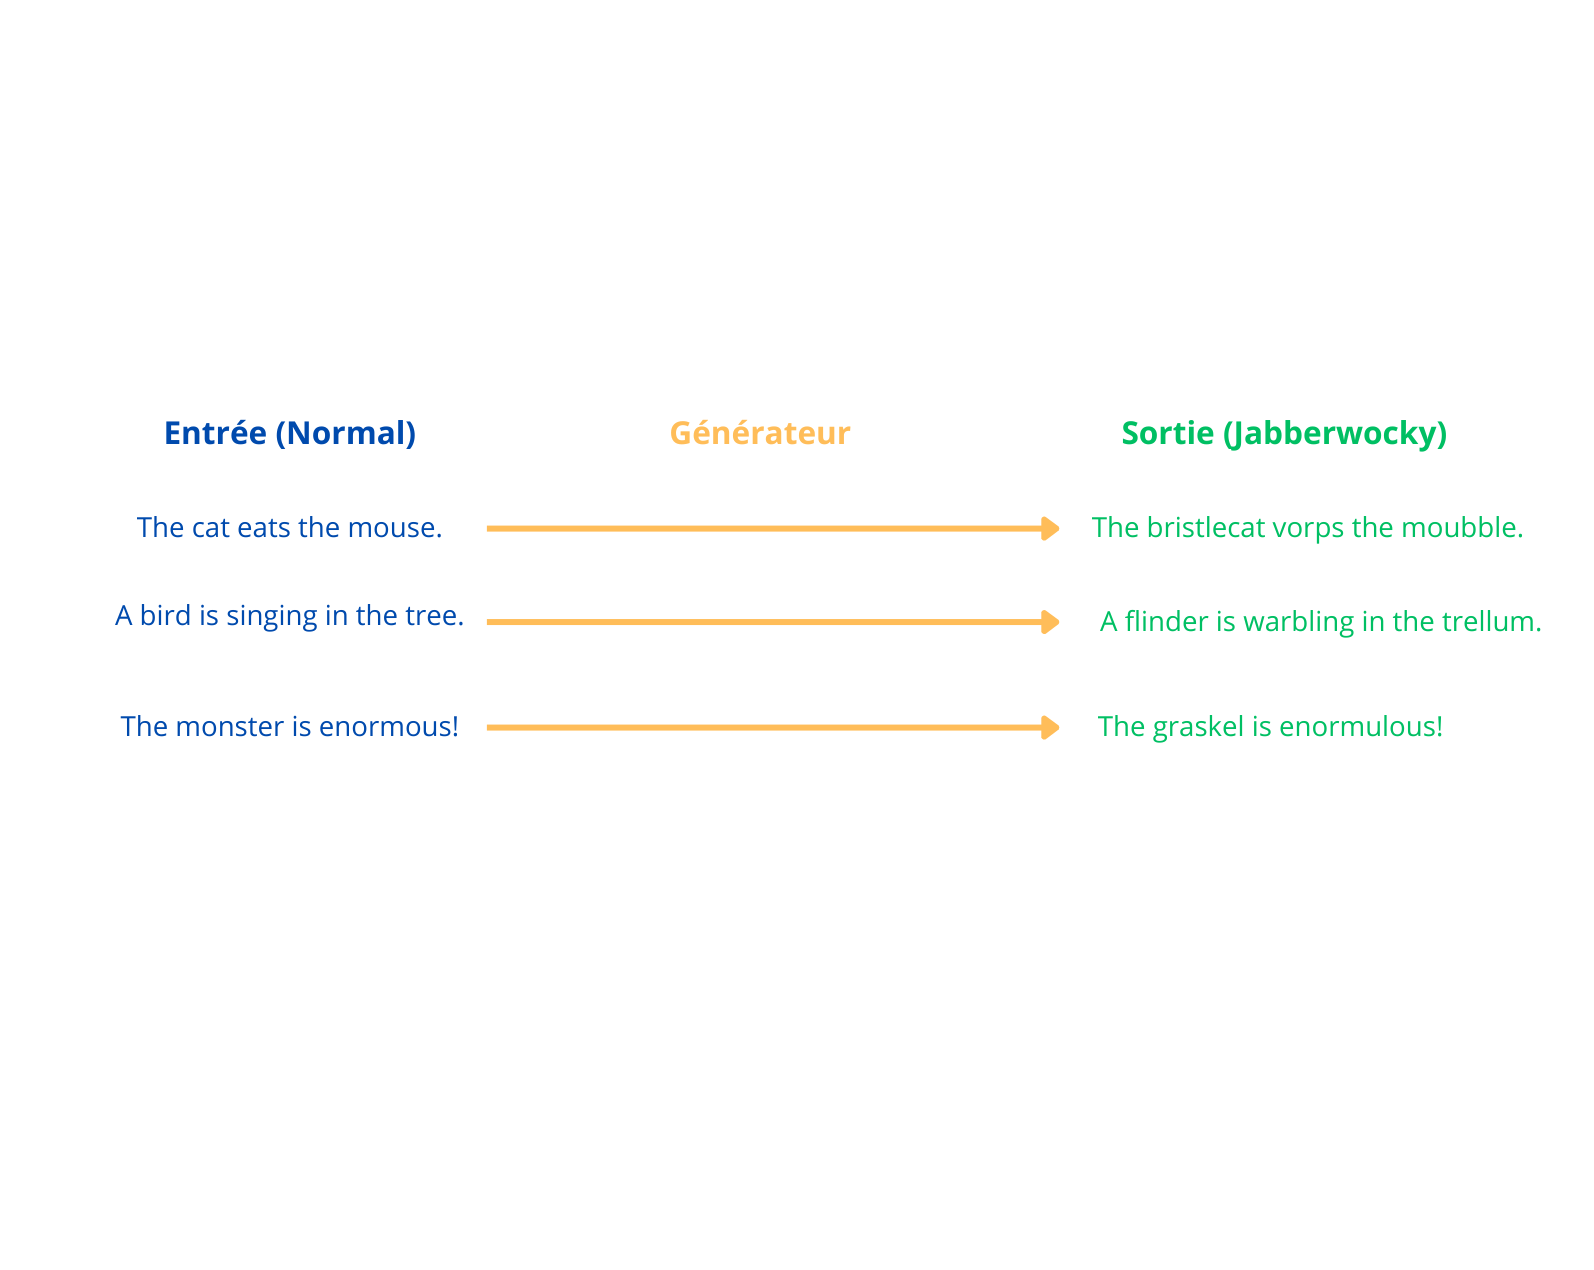
\includegraphics[width=0.9\textwidth]{Le_Jabberwocky_(en).png}
    
    \caption{Illustration du processus de génération des stimuli « Jabberwocky ». Le générateur conserve les mots-outils (en bleu) mais remplace les mots lexicaux par des pseudo-mots (en vert) respectant la phonotactique. \textit{Source : Production personnelle}}
    
    \label{fig:jabberwocky_process}
\end{figure}

\subsection{Validation et tests de TwoNN}
Avant d'analyser les embeddings, nous devons calibrer notre instrument de mesure :
\begin{itemize}
    \item \textbf{Tests de l'algorithme TwoNN} sur des variétés synthétiques dont la dimension est connue (ex: hypersphère). Cela nous permettra d'ajuster les hyperparamètres (nombre de voisins $k$) avant l'application sur les données réelles.
\end{itemize}

\section{Expérimentation Principale (Mars)}

L'objectif de cette phase est de tester les Hypothèses 1 (Ramping) et 2 (Impact Sémantique) définies dans le premier chapitre.

\subsection{Extraction et Tokenisation}
Le traitement des données suivra le protocole suivant :
\begin{itemize}
    \item \textbf{Passage des phrases} dans le tokenizer BPE (Byte Pair Encoding).
    \item \textbf{Normalisation temporelle} : mise en place d'une méthode pour pallier les disparités de longueur des séquences, dues à la fragmentation plus importante des pseudo-mots (Jabberwocky) par le tokenizer.
\end{itemize}

\subsection{Calcul de la Dimensionnalité Intrinsèque}
C'est le cœur de notre expérience technique :
\begin{itemize}
    \item \textbf{Enregistrement des états cachés} (hidden states) couche par couche, lors de l'exécution du modèle (forward pass).
    \item \textbf{Calcul de l'ID via TwoNN} mot après mot (approche incrémentale) pour visualiser la dynamique temporelle de l'intégration de l'information.
\end{itemize}

\subsection{Analyse des profils de « Ramping »}
Une fois les données brutes obtenues, nous passerons à l'analyse :
\begin{itemize}
    \item \textbf{Comparaison statistique} des pentes d'ID entre le groupe Sémantique et le groupe Jabberwocky.
    \item \textbf{Vérification de l'hypothèse} d'une accumulation d'informations (ramping) significativement plus soutenue pour les phrases porteuses de sens.
\end{itemize}

\section{Analyse Structurelle et Extension (Mars)}

Dans cette troisième phase, l'objectif est de tester l'Hypothèse 3 (Profil Hunchback) et de tenter une généralisation des résultats sur une architecture plus récente (Llama 3.1).

\subsection{Étude du profil Hunchback sur GPT-2}
Nous chercherons à valider la théorie de la compression de l'information :
\begin{itemize}
    \item \textbf{Agrégation des IDs moyens} par couche, de l'entrée (embedding layer) à la sortie (prediction head).
    \item \textbf{Identification des phases} d'expansion et de compression caractéristiques du profil Hunchback.
    \item \textbf{Observation des anomalies} : nous analyserons spécifiquement la déformation de ce profil (potentiel échec de compression) sur le dataset Jabberwocky.
\end{itemize}

\subsection{Réplication sur Llama 3.1}
Pour assurer la robustesse de nos conclusions :
\begin{itemize}
    \item \textbf{Adaptation du code} pour gérer l'inférence sur Llama 3.1 (modèle de 8 milliards de paramètres).
    \item \textbf{Comparaison inter-modèles} : nous comparerons les résultats avec GPT-2 pour déterminer si la « profondeur » du modèle ou sa taille influence la vitesse et l'efficacité de la compression sémantique.
\end{itemize}

\section{Interprétation et Rédaction (Avril)}

La phase finale consistera à synthétiser les résultats et à les confronter au modèle neurolinguistique MUC.

\subsection{Visualisation des données}
La production de supports graphiques sera prioritaire pour le rapport final :
\begin{itemize}
    \item \textbf{Création de graphes comparatifs} montrant les courbes d'évolution de l'ID au cours du temps (pour le ramping) et à travers les couches (pour le profil Hunchback).
\end{itemize}

\subsection{Analyse critique}
Enfin, nous rédigerons l'analyse finale :
\begin{itemize}
    \item \textbf{Discussion des résultats} au regard des hypothèses initiales.
    \item \textbf{Traitement des limites} : nous discuterons notamment de l'absence du mécanisme de « Contrôle » (au sens du modèle MUC) dans les modèles de langage actuels et son impact sur le traitement des phrases absurdes.
\end{itemize}